\documentclass[11pt]{article}

\usepackage{graphicx} % See comment above

\textwidth = 6.5 in
\textheight = 9 in
\oddsidemargin = 0.0 in
\evensidemargin = 0.0 in
\topmargin = 0.0 in
\headheight = 0.0 in
\headsep = 0.0 in
%\parskip = 0.2in
\parskip 6pt
\parindent = 0.0in

%\textwidth 6.5in
%\textheight 9in
%\oddsidemargin 0pt
%\evensidemargin 0pt
%\topmargin -.5in
%\headheight .25in

\newtheorem{theorem}{Theorem}
\newtheorem{corollary}[theorem]{Corollary}
\newtheorem{definition}{Definition}
%% Add next two lines for Adobe type fonts! 12/5/01 Tony Seibert
\fontfamily{ptm}\selectfont
\renewcommand{\rmdefault}{ptm}

%\title{Brief Article}
%\author{The Author}
\begin{document}

%\ifpdf
%\DeclareGraphicsExtensions{.pdf, .jpg, .tif}
%\else
%\DeclareGraphicsExtensions{.eps, .jpg}
%\fi

%\maketitle

\title{Lab 7:  Combinatorics}
\author{Physics 116B}
\maketitle
\setcounter{secnumdepth}{2}

\section*{Introduction}

In this lab, you will construct a 2-bit decoder and a 2-bit adder circuit using discrete logic gates.  The parts  you will need
and their pin-outs are shown in the Appendix.

\section*{2-bit Decoder}

Using AND gates and inverters, construct the two-bit digital decoder shown in Figure~\ref{fig:decoder}; that is, a device for which the numerical binary input $i=(A_1A_0)_2$ will cause output $Q_i$, and only that output, to be TRUE (e.g. $A_1=1, A_0=0\rightarrow Q_2=1$).  Use as few devices as possible.  


\begin{figure}[h!]

\centerline{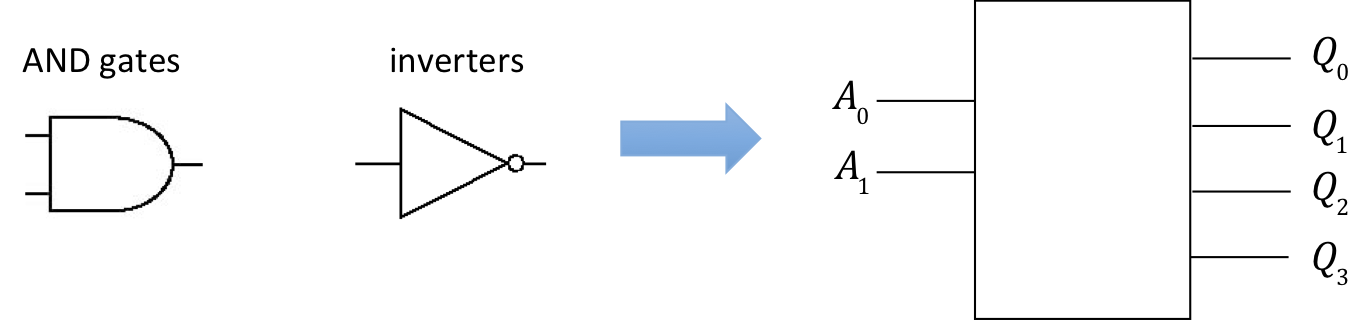
\includegraphics[width=5in]{figs/decoder.png}}
\caption{Two-bit decoder}
\label{fig:decoder}
\end{figure}




Connect the inputs to the logic switches on the proto-boards and the outputs to the LED indicators.

Verify that that the outputs behave as expected for all combinations of the input bits and fill out a truth table with the state of the four outputs for
all possible states of $A_0$ and $A_1$.


\section*{2-bit Adder with Carry Out}

\begin{figure}[h!]

\centerline{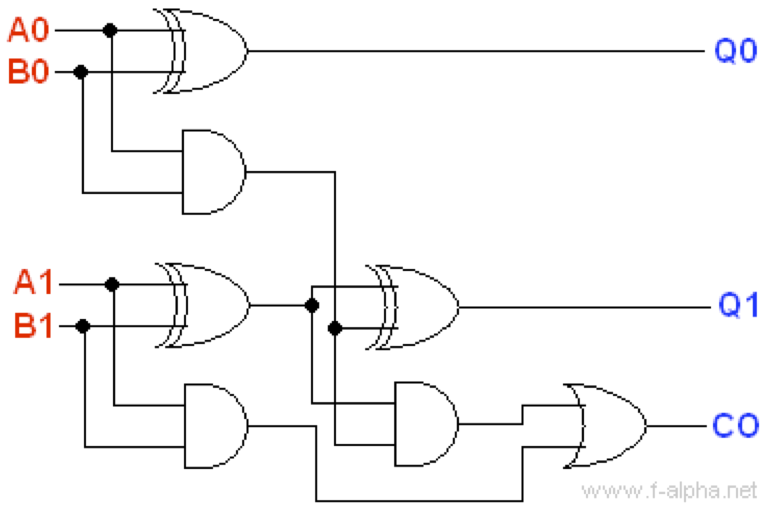
\includegraphics[width=3in]{figs/adder.png}}
\caption{Two-bit adder with carry out.}
\label{fig:adder}
\end{figure}


Wire up the following 2-bit adder circuit shown in Figure~\ref{fig:adder}. Connect the inputs to the logic switches on the proto-board and the outputs to the LED indicators.  


Fill out a truth table for all 16 combinations of the input switches, and verify that the circuit behaves as expected.

Disconnect the $A_0$ bit from the switch and connect it to the TTL function generator.  Set bit $A_1$ to 0 and $B_0$ and $B_1$ to 1.  Measure the propagation delay from $A_0$ changing state (both high and low) to $Q_0$, $Q_1$, and $CO$ reaching their final values.  Include the appropriate scope traces in your lab report.




\section*{Appendix: Chips Used in this Lab}

\vskip 2 cm

\begin{centering}

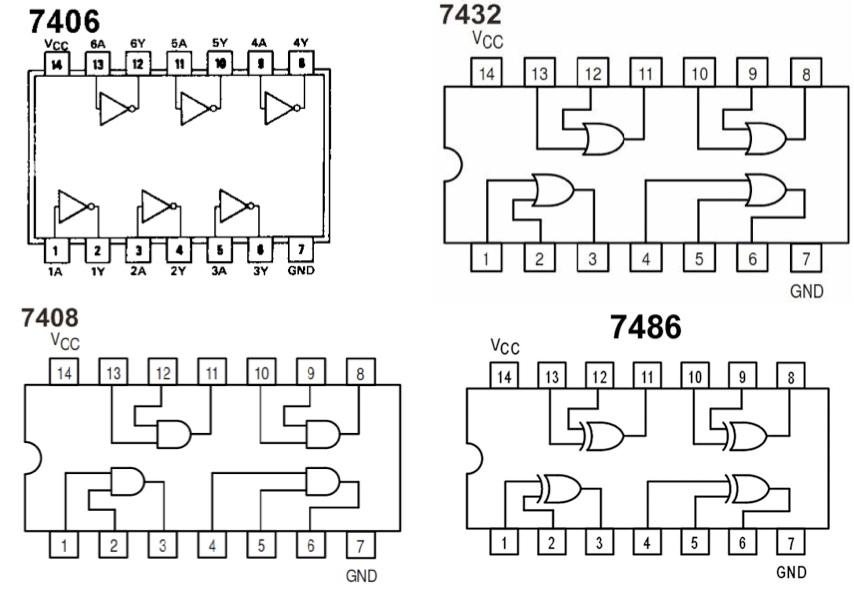
\includegraphics[width=5 in]{figs/gates.png}

\end{centering}

\end{document}

